\titleformat{\chapter}
{\normalfont\fontsize{12}{15}\centering}{Anexos \thechapter.}{0.3em}{}[]

\clearpage
\thispagestyle{empty}
\begin{center}
  \vspace*{\fill}
  \phantomsection
  Apéndices
  \addcontentsline{toc}{chapter}{Anexos}
  \vspace*{\fill}
\end{center}
\clearpage

\appendix
\uextra{Apendice}{Dispositivo Raspberry Pi 4 Model B}
\begin{figure}[h!]
  \centering
  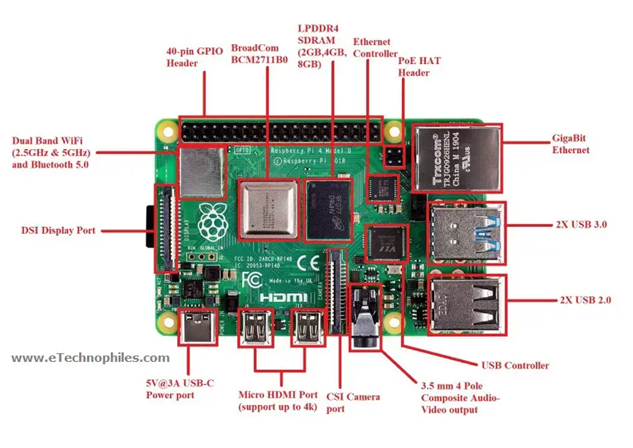
\includegraphics[width=0.95\textwidth]{Anexos/1.arquitectura-raspberry.png}
  \caption{Arquitectura del Raspberry Pi 4 Model B}
  \label{fig:raspberry-architecture}
\end{figure}

\uextra{Apendice}{Verificación del sistema de monitoreo acústico}

{\small
  \begin{longtable}[c]{c p{3.5cm} p{2.2cm} p{2.2cm} p{3.5cm}}
    \hline
    \textbf{Requerimiento} & \textbf{Descripción}                                                                                    & \textbf{Entrada}                                                  & \textbf{Salida}                                                       & \textbf{Criterio de Aceptación}                                                       \\
    \hline
    \endfirsthead

    \hline
    \textbf{Requerimiento} & \textbf{Descripción}                                                                                    & \textbf{Entrada}                                                  & \textbf{Salida}                                                       & \textbf{Criterio de Aceptación}                                                       \\
    \hline
    \endhead
    \endfoot
    \endlastfoot

    R1                     & Captura continua del audio ambiental a través de micrófonos.                                            & Señales de audio del entorno a través del hardware del micrófono. & Eventos discretos etiquedados del audio.                              & El sistema debe estar activo y registrando datos en todo momento.                     \\
    \addlinespace
    R2                     & Procesamiento del audio para clasificarlo en eventos sonoros predefinidos.                              & Flujo de datos de audio.                                          & Clasificación del sonido (ej. voz, silencio, golpe).                  & El sistema debe etiquetar correctamente la señal de audio que recibe en todo momento. \\
    \addlinespace
    R3                     & El sistema debe conocer en todo momento el estado de actividad del entorno.                             & Señal de audio.                                                   & Hay ruido o silencio.                                                 & El sistema reconoce cuando hay ruido o silencio.                                      \\
    \addlinespace
    R4                     & Comparación de la actividad en tiempo real con el perfil de normalidad para detectar patrones anómalos. & Secuencia de eventos en tiempo real                               & Identificación de una anomalía o evento atípico.                      & Detectar si una secuencia de eventos es normal o anómala.                             \\
    \addlinespace
    R5                     & El sistema realiza una consulta verbal al usuario al detectar una anomalía.                             & Señal de audio.                                                   & Emisión de una pregunta de voz pregrabada (ej. ``¿Está todo bien?''). & El sistema consulta el estado del usuario antes de enviar una alerta.                 \\
    \addlinespace
    R6                     & Permitir cancelar una alerta de emergencia por comando de voz.                                          & Respuesta de voz del usuario (ej. ``Estoy bien'').                & No se envía alerta.                                                   & El sistema cancela la alerta.                                                         \\
    \addlinespace
    R7                     & El sistema envía notificaciones de emergencia si la anomalía es crítica o el usuario no responde.       & Falta de respuesta del usuario o gravedad de la anomalía          & Envío de notificaciones.                                              & El sistema es capaz de enviar una alerta sin la intervención del usuario.             \\
    \bottomrule
    \addlinespace

    \caption{Requerimientos del sistema acústico}
    \label{tab:requerimientos_sistema_acustico}
  \end{longtable}
}
